\documentclass{acm_proc_article-sp}

\usepackage{graphicx,url}
\usepackage{listings}
\usepackage{subfigure}
\usepackage{multirow}
\usepackage{pictexwd}
\usepackage[absolute]{textpos}
\usepackage[english]{babel}
   
\lstset{%
  keywordstyle=\bfseries,
  aboveskip=15pt,
  belowskip=15pt,
  captionpos=b,
  identifierstyle=\ttfamily,
  escapeinside={(*@}{@*)},
  stringstyle=\ttfamiliy,
  %frame=single,
  numbers=left, basicstyle=\scriptsize, numberstyle=\tiny, stepnumber=0, numbersep=2pt}

\newcommand{\prg}[3][tbp]{
\begin{figure}[#1]
  \lstinputlisting[language=C,keywordstyle=\bfseries,
  aboveskip=15pt,
  belowskip=15pt,
  captionpos=b,
  identifierstyle=\ttfamily,
  escapeinside={(*@}{@*)},
  stringstyle=\ttfamiliy,
  frame=single,
  numbers=left, basicstyle=\tiny, numberstyle=\tiny, stepnumber=0, numbersep=2pt]{fig/#2.cc}
  \caption{#3}
  \label{prg:#2}
\end{figure}
}

\newcommand{\prgFull}[3][tbp]{
  \lstinputlisting[language=C,keywordstyle=\bfseries,
  aboveskip=15pt, 
  belowskip=15pt,
  captionpos=b,
  identifierstyle=\ttfamily,
  escapeinside={(*@}{@*)},
  stringstyle=\ttfamiliy,
  %frame=tbrl,
  numbers=left, basicstyle=\tiny, numberstyle=\tiny, stepnumber=0, numbersep=2pt]{fig/#2.cc}
}


\newcommand{\tab}[3][ph]{
  \begin{table}[#1]
    {\centering\small\textsf{\input{fig/#2.tab}}\par}
    \caption{#3}
  \label{tab:#2}
  \end{table}
}

\newcommand{\fig}[4][ht!]{
  \begin{figure}[#1]
    {\centering{\includegraphics[#4]{fig/#2}}\par}
    \caption{#3}
    \label{fig:#2}
  \end{figure}
}


\newcommand{\Fig}[4][hp]{
  \begin{figure*}[#1]
    {\centering{\includegraphics[#4]{fig/#2}}\par}
    \caption{#3}
    \label{fig:#2}
  \end{figure*}
}

\def\sharedaffiliation{%
\end{tabular}
\begin{tabular}{cc}}
	
\hyphenation{sche-du-ling}

\begin{document}

\title{The Real Influence of Shared Memory Contention on Real-time Multicore Applications}


\numberofauthors{4}
\author{
\alignauthor Giovani Gracioli$^{1}$\\
       \email{giovani@lisha.ufsc.br}
% 2nd. author
\alignauthor Julio Sincero$^{2}$\\
       \email{sincero@cs.fau.de}
\and
% 3rd. author
\alignauthor Wolfgang Schr\"{o}der-Preikschat$^{2}$\\
       \email{wosch@cs.fau.de}
% 4th. author
\alignauthor Ant\^{o}nio Augusto Fr\"{o}hlich$^{1}$\\
       \email{guto@lisha.ufsc.br}
%
	\sharedaffiliation
	\affaddr{$^{1}$Software/Hardware Integration Lab} & \affaddr{$^{2}$Department of Computer Science 4}\\
    \affaddr{Federal University of Santa Catarina} & \affaddr{Friedrich-Alexander University Erlangen-Nuremberg}\\
    \affaddr{Florian\'{o}polis, Brazil} & \affaddr{Erlangen, Germany}\\
}

\maketitle

\begin{abstract}
The continuous evolution of processor technology has allowed the utilization of multicore architectures in the embedded system domain. A major part of embedded systems, however, are inherently real-time (soft and hard) and the use of multicores in this domain is not straightforward due to their unpredictability in bounding worst case execution scenarios. One of the main factors for unpredictability is the coherence through memory hierarchy. This paper characterizes the real influence of contention for shared data memory in the context of embedded real-time applications. By using a worst-case benchmark, we have measured the real impact of excessive shared memory invalidations on five processors with three different cache-coherence protocols (MESI, MOESI, and MESIF) and two memory organization (UMA and ccNUMA). Results have shown that the execution time of an application is affected by the contention for shared memory (up to 3.8 times slower). Towards a solution, we propose an architecture composed by several OS techniques, such as memory partitioning and scheduling. We also provide an analysis on Hardware Performance Counters (HPC) and propose to use them in order to monitor and detect excessive memory invalidations at run-time.
\end{abstract}

\category{C.3}{Special-Purpose and Application-Based Systems}{Real-time
  and embedded systems}

\terms{Design, Experimentation}

\keywords{Contention for shared data memory, Real-time scheduling, Multicore processors}

\section{Introduction}

Several embedded real-time applications are implemented in a dedicated hardware logic (i.e. \textit{Application-Specific Integrated Circuit - ASIC}) to obtain maximum performance and fulfill all application's requirements (processing, real-time deadlines, etc). For instance, digital signal processing algorithms and baseband processing in wireless communication, should process a big amount of data under real-time conditions. Nevertheless, as they are usually implemented in a dedicated hardware, these applications present restrictions in terms of developing support (e.g. bug fixes, updating, maintainability).

The continuous evolution of processor technology, however, together with its decreasingly cost, has enabled multicore (e.g. \textit{Symmetric Multiprocessing - SMP}) architectures to be also used in the embedded real-time system domain~\cite{Cho2006}. Thus, the same applications can be ported to software, with similar performance and more support flexibility to their developers. In this context, an application is implemented on top of a Real-Time Operating System (RTOS), composed by several real-time cooperating threads (threads that share data). 

In this scenario, due to multicore processor organization, some important characteristics must be considered, specifically, the memory hierarchy~\cite{Muralidhara:2010, Zhuravlev:2010}. The memory hierarchy holds an important role, because it affects the estimation of the Worst-Case Execution Time (WCET), which is extremely important in the sense of guaranteeing that all threads will meet their deadlines through the design phase evaluation (schedulability analysis)~\cite{Marwedel2005, Suhendra2008}.

Several works have been proposed to deal with memory organization in multicore architectures and provide real-time guarantees~\cite{Anderson2009a, Anderson2008, Anderson2006, Cho2006}, but they only consider scenarios where threads are independent, that is, there is no sharing of data. In this case, the influence among threads (contention for cache space and interference in the cache lines) can be solved by some memory partitioning/locking mechanism provided by a special hardware~\cite{Suhendra2008} or implemented into the (real-time) scheduler~\cite{Guan2009, Zhuravlev:2010}. Partitioning/Locking techniques avoid overlapping of shared cache spaces and reduce the contention for the shared resource, increasing the application's throughput.

In situations where threads share data in a cooperating fashion, a partitioning/locking mechanism does not avoid the contention for shared data. For instance, consider a scenario composed by ``n" threads sharing data, running on ``m" cores in a pipeline order (thread 2 after thread 1, thread 3 after thread 2, and so on), as demonstrated in Figure~\ref{fig:coop_threads}. Thread 1 executes and writes in the shared data location. When the thread 2 accesses the shared data, it gets an invalid access and must ask (snoop request) for the most recent copy of the data or recover it from a lower memory level (previous cache level or main memory). The task of performing a snoop request, in the current SMP processors, is done automatically by the memory controller hardware, which increases the threads' execution time, even without their knowledge. The time to complete a snoop request is considerably slow (comparable to access the off-chip RAM)~\cite{BoydWickizer:10}, which can lead to an unexpected increase of the thread's execution time and, in case of a real-time application, to deadline losses. 

\fig{coop_threads}{An example of pipeline application composed by threads sharing data.}{scale=.6}

In this paper, we bring the problem of contention for shared memory to the embedded real-time system domain by measuring its real influence on five different modern processors with three different cache-coherence protocols (MESI, MOESI, and MESIF) and two memory organization (UMA and ccNUMA). We use a benchmark composed by two versions of the same application -- sequential and parallel -- for comparison purpose. Common sense dictates that the parallel version should run about two times faster than the sequential one. Consequently, if the sequential version is schedulable (proved by a schedulability analysis), the parallel version should be schedulable as well. We demonstrate in our experiments that due to the current multicore memory organization,
the parallel version has its execution time affected (up to 3.8 times slower), which can lead to deadline losses. Towards a solution, we envision an environment where the operating system (OS) real-time scheduler, together with a memory partitioning and Hardware Performance Counters (HPCs) support, could detect excessive memory invalidations between threads and take a decision (scheduling) in order to avoid deadline losses. Scheduling is a good solution because it does not require special hardware support and is easily integrated in practically any RTOS~\cite{Zhuravlev:2010}. Moreover, the scheduler is completely transparent to applications, that is, there is no need to change the application source code neither OS APIs nor libraries.

In summary, in this paper, we make the following contributions:

\begin{itemize}
	\item We motivate the problem by measuring the real influence of contention for shared memory in the context of real-time applications where deadlines must be always met.
	\item We evaluate the problem on five different multicore processors, with three different cache-coherence protocols (MESI, MOESI, and MESIF) and two memory organization (UMA and ccNUMA) by using a benchmark composed by a sequential and parallel version of the same application.
	%\item We review the correlated state-of-art areas.
	\item Towards the problem solution we propose an architecture composed by OS techniques, such as scheduling, HPCs, and memory partitioning, in order to provide predictability and real-time guarantees. Moreover, we evaluate HPCs in one of the five processors. HPCs can be used to monitor and detect when two or more threads are sharing data. HPCs together with the OS scheduler and memory partitioning are good alternatives to decrease the contention for shared data memory and provide predictability and performance gains to real-time applications.
\end{itemize}

The remainder of this paper is organized as follows. Section~\ref{sec:back} summarizes the background needed to follow the rest of the paper. In Section~\ref{sec:problem}, we describe in details the problem that we are addressing. The benchmark evaluation is presented in Section~\ref{sec:benchmark}. Section~\ref{sec:disc} discusses the results. Section~\ref{sec:related} provides an overview of previous work on memory hierarchy in multicore architectures and memory-aware and real-time multicore scheduling. Finally, Section~\ref{sec:conc} concludes the paper.

\section{Background}
\label{sec:back}

\subsection{Cache-coherence Protocols}

In SMP systems, each processor fetches its own instructions and operate its own data, characterizing a Multiple Instruction Multiple Data (MIMD) system. They feature a unique shared Uniform Memory Access (UMA) or a cache-coherent Non-Uniform Memory Access (ccNUMA), easing data sharing. Two memory organization widely used in today's SMP processors are presented in Figure~\ref{fig:caches}. In Figure~\ref{fig:cache1}, ``n" cores have a private level 1 cache, share a larger level 2 cache and the main memory. An example of processor that uses this architecture is the Intel dual-core Q9550. Figure~\ref{fig:cache2} shows another memory hierarchy. There are two physical dies, where each one is composed by two cores. Each core has a private L1 cache, each die shares a L2 cache, and a L3 cache and main memory are shared by all cores. Intel Xeon L7455 with 24 cores and 6 dies is an example of this architecture. Note that there are variations from these two architectures (e.g. \textit{Symmetric Multithreading - SMT}, L2 shared cache for all dies, etc), but the same principle of sharing the lower levels of memory still applies.

\begin{figure}[htb]
\centering
\subfigure[] {
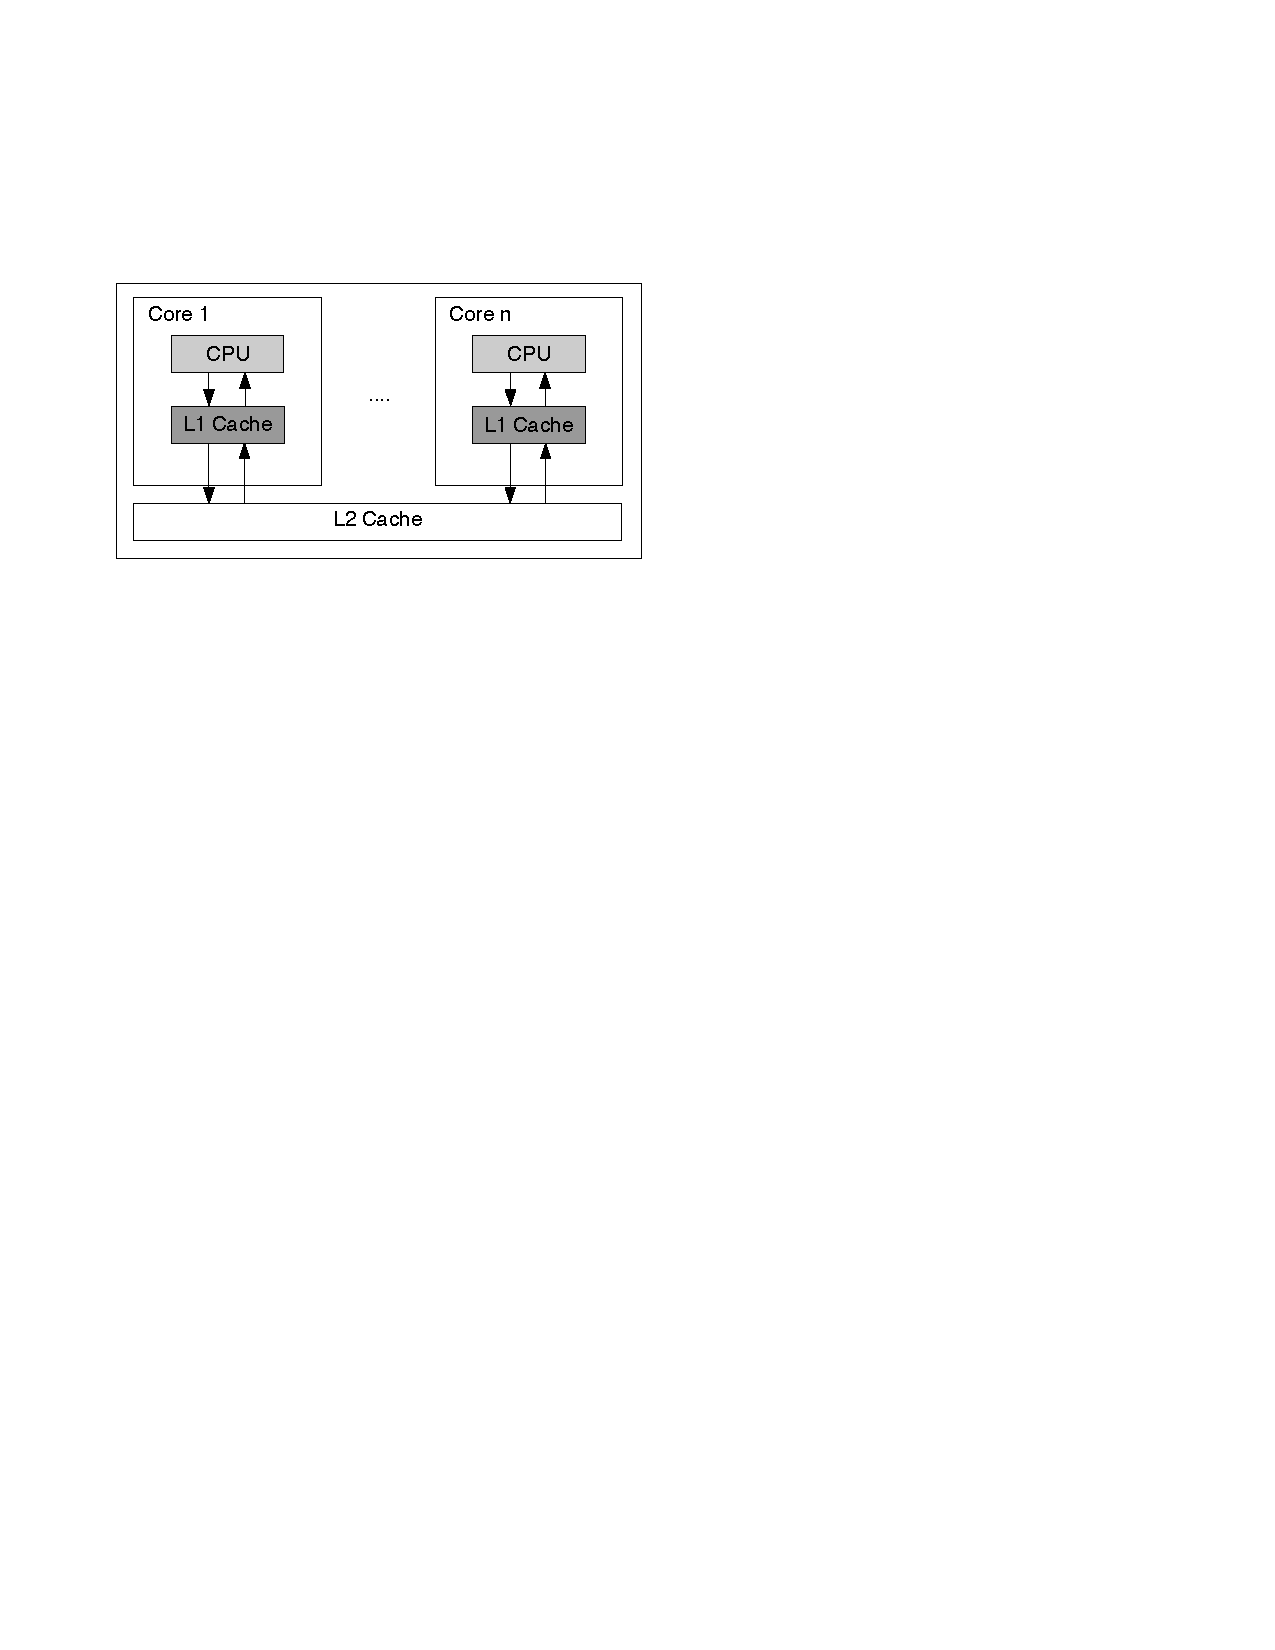
\includegraphics[scale=.6]{fig/cache_arch1}
\label{fig:cache1}
}
\subfigure[] {
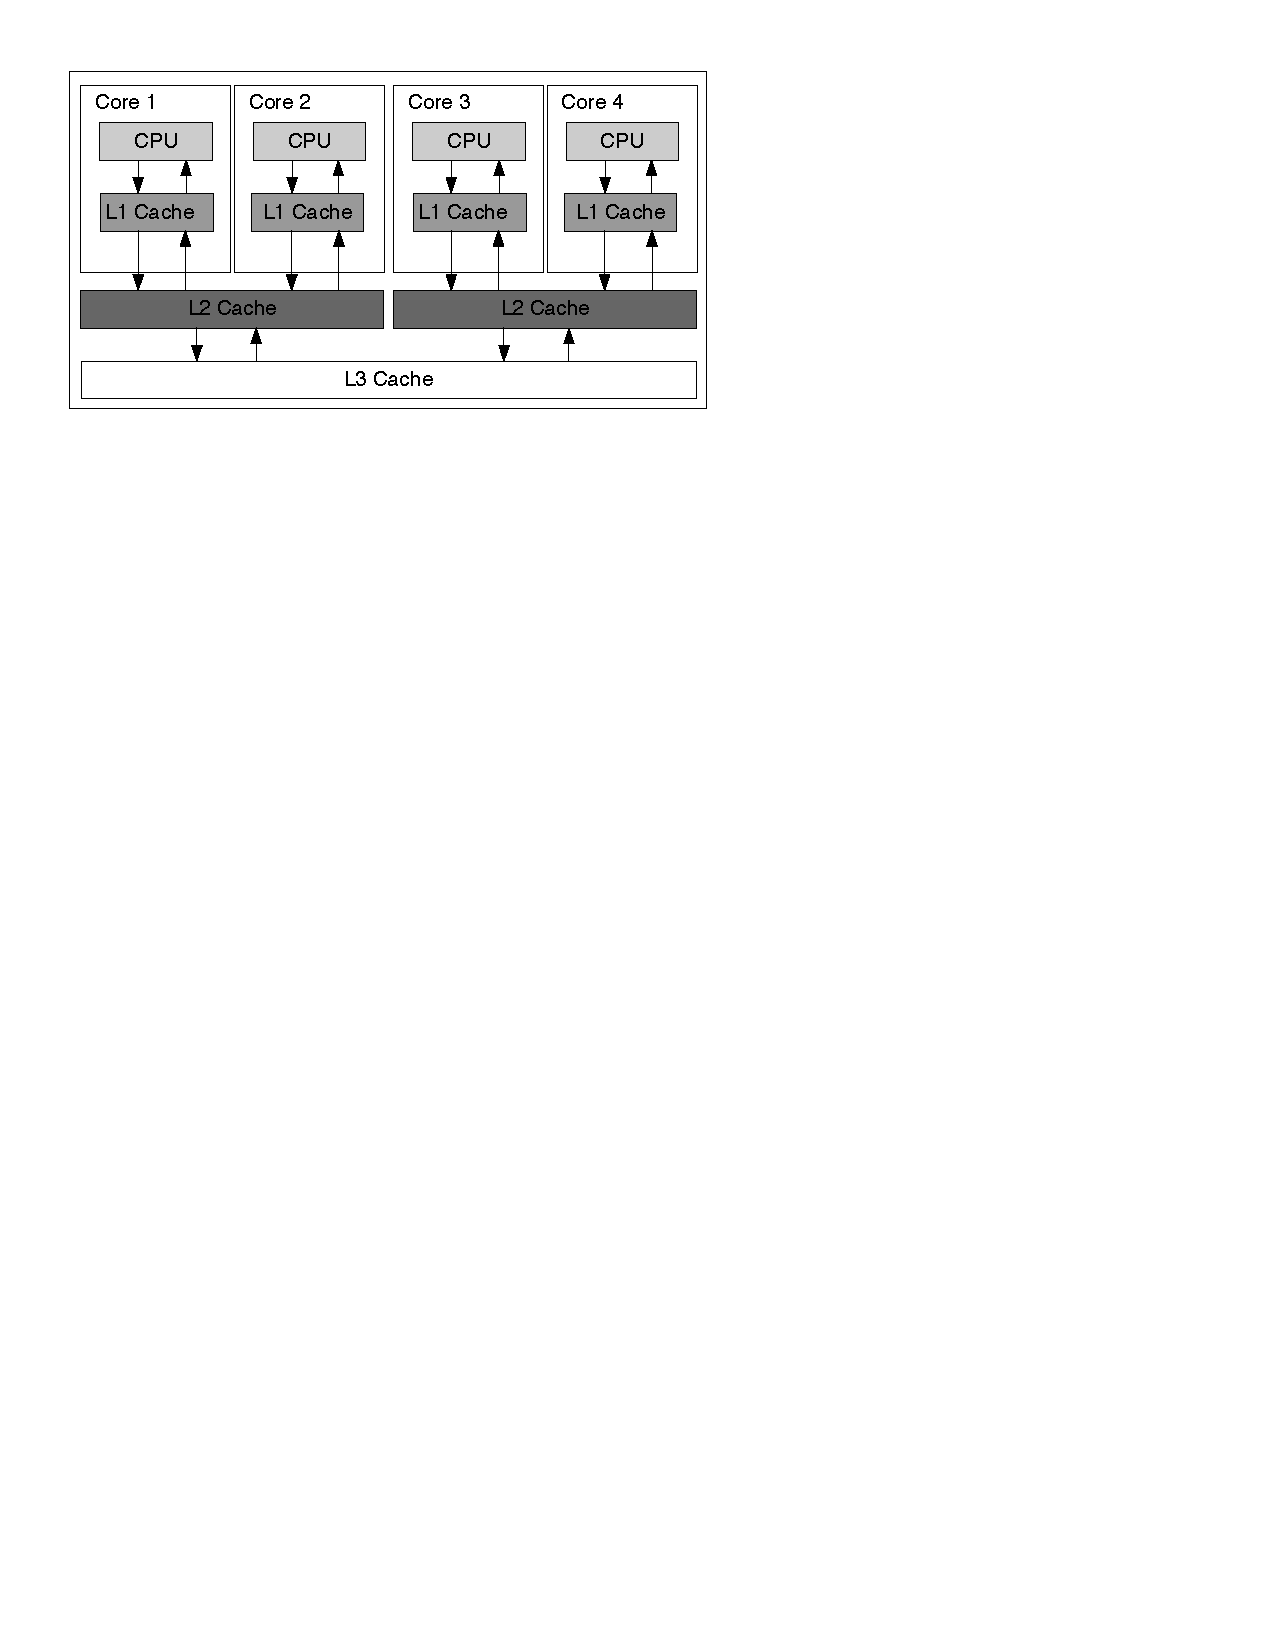
\includegraphics[scale=.5]{fig/cache_arch2}
\label{fig:cache2}
}
\caption{(a) An architecture with shared level-2 cache. (b) An architecture with a cluster sharing level-2 and all cores sharing the level-3.}
\label{fig:caches}
\end{figure}

Shared memory consistency between cores is normally supported by the hardware through bus snooping and cache-coherence protocol. It means that every core snoops the bus to determine if it has a copy of the data that is being requested. The MESI protocol is the most common cache-coherence protocol which supports write-back cache~\cite{Patterson:06}. In a write-back cache, writes are not immediately forwarded to the main memory, instead the written locations are marked as dirty. Data in these locations are written back to the memory when they are evicted from the cache. Thus, a read miss in a write-back cache requires two memory accesses: one to retrieve the needed data and one to write replaced data from cache to the store location. In the MESI protocol, every cache line is marked with one of the four states: 

\begin{itemize}
\item \textbf{Modified (M)}: the cache line is present only in the current cache and its data is dirty. The value must be written to the memory before a reading. The write-back changes the state to exclusive.
\item \textbf{Exclusive (E)}: the cache line is present only in the current cache and it is clean. The state can be changed to the Shared state when a read request from another core arrives or to Modified state when a write operation is performed.
\item \textbf{Shared (S)}: indicates that the cache line is shared by other caches and its state is clean. 
\item \textbf{Invalid (I)}: a cache line in this state does not hold a valid copy of data. The valid data can be in the main memory or in another processor cache.
\end{itemize}

The MOESI protocol adds a fifth state to the MESI protocol~\cite{amd64}. The \textbf{Owned (O)} state represents data that is both modified and shared. This avoids the need to write modified data back to the main memory before sharing it. Only one processor can hold a cache line in the Owned state -- the same cache line in other processors must be in the shared state. The processor which holds a cache line in the Owned state is the only one to respond to a snoop request. When a snoop request arrives, the cache line switches to the Owned state, and the duplicate copy is made in the S state. As a result, any cache line in the O state must be written back to memory before it can be evicted, and the S state no longer implies that the cache line is clean. 
%In comparison, a system using MESIF or MESI would change the cache line to the F or S state, copy it to the requesting cache and write the data back to memory -- the O state avoids the write back, saving some bandwidth.

%However, there is at least one optimization which Intel did not pursue -- the Owner state that is used in the MOESI protocol (found in the AMD Opteron). The O state is used to share dirty cache lines (i.e. lines that have been written to, where memory has older or dirty data), without writing back to memory. 
The MESIF protocol includes a \textbf{Forward (F)} state that is used to respond to request for a copy of a cache line~\cite{intel}. The newly created copy is placed in the F state and the cache line previously in the F state is put in the Shared (S) state or in the Invalid (I) state. Thus, there is only one copy in the F state and the remaining copies are in the S state. MESIF and MOESI protocols are usually used in ccNUMA architectures, such as Intel Nehalem and AMD Opteron respectively, while MESI is widely used in UMA architectures, such as Intel dual-core.
%The F state is different from the O state of MOESI protocol, in that the processor having data in the O state has the only updated data value in the memory system. This implies that the processor, upon eviction of an owned data, has to send that data back to be stored in the main memory. The F state indicates that the data value is consistent with the copy in the memory system.

\subsection{Hardware Performance Counters}

HPCs are special registers available in the most modern microprocessors through the hardware Performance Monitoring Unit (PMU). HPCs offer support to counting or sampling several micro-architectural events, such as cache misses and instructions counting, in real-time~\cite{Sprunt:02}. However, they are difficult to use due to the limited hardware resources (for example Intel Nehalem supports event counting with seven event counters and AMD Opteron provides four HPC to measure hardware events) and complex interface (e.g. low-level and specific to micro-architecture implementation)~\cite{Azimi:2005}.

Nevertheless, it is possible to use multiplexing techniques in order to overcome the limitation in the number of HPCs~\cite{May:01, Sprunt:02} or specific libraries that make the use of HPCs easier~\cite{Dongarra:2003}, yet adding a low overhead to the application. HPCs can be used together with OS techniques, such as scheduling and memory management, to monitor and identify performance bottlenecks in order to perform dynamic optimizations~\cite{Azimi:2009}. In multicore systems, for instance, it is possible to count the numbers of snoop requests, last-level cache misses, and evicted cache lines. 
%In the next section, we describe the problem related to the shared memory coherence.

\section{Problem Description}
\label{sec:problem}

The problem we are addressing in this paper raises from the memory hierarchies present in the today's SMP architectures (see Figure~\ref{fig:caches}) and their memory coherence protocols. Each core has its own data and uses its private data cache for speeding up the processing. However, when cores share data, each copy of the data is placed in the core's private cache and the cache-coherence protocol is responsible for keeping the consistency between each copy.

When a core writes into a data that other cores have cached, the cache-coherence protocol invalidates all copies, causing an implicit delay in the application's execution time. At the same way, when a core reads a shared data that was just written by another core, the cache-coherence protocol does not return the data until it finds the cache that has the data, annotate that cache line to indicate that there is shared data, and recover the data to the reading core. These operations are performed automatically by the hardware and take hundreds of cycles (about the same time as accessing the off-chip RAM), increasing the application's execution time~\cite{BoydWickizer:10}. Two kinds of scaling problem occur due to shared memory contention~\cite{BoydWickizer:10}: access serialization to the same cache line done by the cache coherence protocol, which prevent parallel speedup, and saturation into the inter-core interconnection, also preventing parallel processing gains.

%As an example, consider a scenario where "n" threads are executed in different cores in a pipeline order, sharing data, as demonstrated by Figure~\ref{fig:coop_threads}. Thread 1 executes and writes into the shared data location. When thread 2 accesses the same data, it gets an invalid access (a cache line invalidation), and the data should be recovered from the other core's cache or from the lower memory level before reading/writing from/to data. When the next threads run, the same problem occurs, which increases the final application's execution time.

%Bringing this problem to the real-time domain, 
The contention for shared memory causes an increase in the application's throughput and deadline losses. One can argue that there would be processing speedup by just turning the cache off and using the main memory directly. Nevertheless, it is misconception that worst-case execution times with caches are equal to ones without caches~\cite{Liedtke:1997}. Moreover, it is common to find a considerable inter-thread interaction in multithreaded application. For example, some applications from NAS parallel and SPEC OMG benchmark suites have up to 20\% of inter-thread interaction, and up to 60\% of this interaction is affected by cache line contention~\cite{Muralidhara:2010}. Reducing the effects of cache line contention can significantly improve the application's overall performance and avoid deadline misses. In the next section we provide an analysis of the described problem by measuring the real influence of shared memory contention through a benchmark.

\section{Problem Evaluation}
\label{sec:benchmark}

In order to evaluate the influence of contention for shared memory data in the execution time of an application, we have designed a worst-case benchmark composed by two versions of a pipeline application and a best-case application for comparing purposes (Figure~\ref{fig:apps}):

\begin{itemize}
 \item \textbf{Sequential}: in this version, two functions are executed in a sequential order. There are no memory conflicts (Figure~\ref{fig:sequential}). The objective of this version is to simulate an algorithm implemented in hardware, that is, the algorithm does not face the shared memory invalidation problem.

 \item \textbf{Parallel}: two threads run at the same time and share data (Figure~\ref{fig:parallel}). The objective of this version is to evaluate the performance of the previous version when it is implemented in a multicore architecture. Common sense dictates that this version should run about two times faster than the sequential one. Consequently, if the sequential version is schedulable (proved by a schedulability analysis), the parallel version should be schedulable as well. We do not use any kind of synchronization (i.e semaphores, mutexes, or condition variables) to ensure the data consistency because we are only interested in measuring the shared data contention overhead.

 \item \textbf{Best-case application}: two threads run at the same time, but do not share data (Figure~\ref{fig:best-case}). Obviously, this application should run about 2 times faster than the sequential one in a multicore processor. The objective is to have a best-case scenario comparable to the sequential and parallel versions.
\end{itemize}

\begin{figure}
\centering
\begin{tabular}{cc}
	\subfigure[] {
	\fbox{
	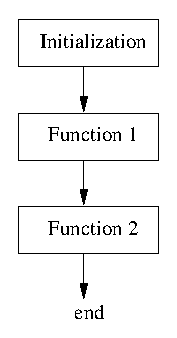
\includegraphics[scale=.6]{fig/seq_app}
	\label{fig:sequential}}} &
	\subfigure[] {
	\fbox{
	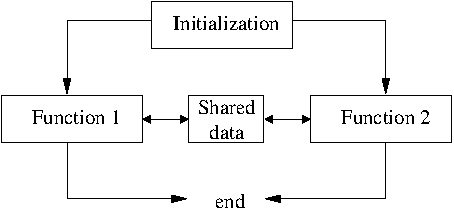
\includegraphics[scale=.6]{fig/par_app}
	\label{fig:parallel}
	}
	}\\
\multicolumn{2}{c}{
\subfigure[] {
\fbox{
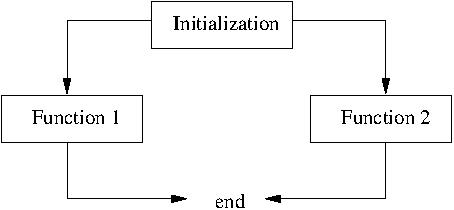
\includegraphics[scale=.6]{fig/best_case_app}
\label{fig:best-case}
}
}
} \\
\end{tabular}
\caption{Benchmark applications: (a) sequential (b) parallel (c) best-case.}
\label{fig:apps}
\end{figure}

All three applications have two two-dimensional arrays of size ROWS x COLS and a loop of 10000 repetitions, in which math operations are executed. The shared data in the parallel version is accessed by reading and writing in both arrays and in the same positions, thus we are sure that both threads are accessing the corresponding cache line. At initialization phase, the arrays are started with zero and the threads are created (parallel and best-case applications). The benchmark was implemented as a Linux application, in C++ (g++ compiler with no optimization flags), and using the pthread library for the parallel and best-case versions. We ran each version in five different processors (Table~\ref{tab:processors}), varying the arrays' size.

\begin{table*}
\begin{center}
\footnotesize{
\begin{tabular}{|c|c|c|c|c|c|}
\hline
\textbf{Feature / Processor} & \textbf{Opteron 280} & \textbf{Intel i5-650} & \textbf{Intel Q9550} & \textbf{Xeon 5030} & \textbf{PowerPC} \\
\hline
Frequency & 2.4 Ghz & 3.2 Ghz &  2.83 Ghz & 2.66 Ghz & 3.2 Ghz\\
\hline
Instruction set & 64 bits & 64 bits & 64 bits & 64 bits & 64 bits \\
\hline
Physical dies & 2 & 1 & 1 & 2 & 1\\
\hline
Cores per die & 2 & 2 & 4 & 2 & 2\\
\hline
SMT & - & 2 & - & 2 & -\\
\hline
Bus Speed & HyperTransport 1.0 Ghz & QPI 1.3 Ghz & FSB 1.3 Ghz & FSB 667 Mhz & 1.6 Ghz\\
\hline
L1 private data & 128 KB 2-way & 32 KB &  64 KB & 16 KB & 32 KB \\
cache size 		& associative  & 	   & 		&	    &		\\  				
\hline
L2 cache  & 1 MB 16-way  & 256 KB per 	   &  12 MB & 4 MB 8-way  & 512 KB\\ 
size 	  & associative  & core (private)  &  		& associative & 	  \\
\hline
L3 shared & - & 4 MB & - & - & - \\
\hline
Cache alignment & 64 bytes & 64 bytes & 64 bytes & 128 bytes & 64 bytes \\
\hline
Memory			& ccNUMA   & ccNUMA	  & UMA & UMA & UMA\\
architecture 	&		   & 		  & 	&	  &	   \\
\hline
Coherence & MOESI & MESIF & MESI & MESI & MESI \\
protocol  &		  &		  &		 &		&	   \\
\hline
Linux version & 2.6.32 & 2.6.32 & 2.6.32 & 2.6.32 & 2.6.32 \\
\hline
Price & \$270.00 & \$ & & & \\
\hline
\end{tabular}
}
\end{center}
\caption{AMD Opteron 280, Intel i5-650, Intel Q9550, Intel Xeon 5030, and PowerPC-based on Cell processors configurations.}
\label{tab:processors}	
\end{table*}

Figure~\ref{fig:q9550_eval} presents the WCET (in logarithm scale) for each application version on the Intel dual-core Q9550 processor. We ran each application for 10 times and then extracted the WCET. The values were measured by the Linux \emph{time} tool. We note that, independently of the arrays' size, the parallel version was always slower than the sequential version (up to 1.31 time). As expected, the best-case application was about 2 times faster than the sequential one. In addition, we repeated the evaluation using an optimized version of the Linux kernel~\cite{BoydWickizer:10}. Basically, the Linux was modified to avoid locks and atomic instructions by reengineering data structures and unnecessary sharing. Figure~\ref{fig:q9550_opt} shows the measured WCET. All applications presented similar performance, and the parallel version was always slower than the sequential one. This performance degradation is caused by the shared memory invalidations (e.g. bus snooping and MESI cache-coherence protocol), which imply in deadline misses considering the embedded real-time domain.

\begin{figure}[htb]
\centering
\subfigure[] {
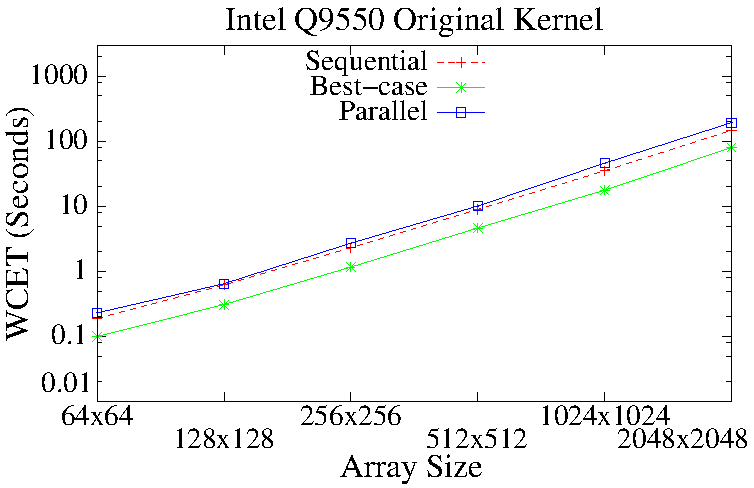
\includegraphics[scale=.4]{fig/q9550_original}
\label{fig:q9550_orig}
}
\subfigure[] {
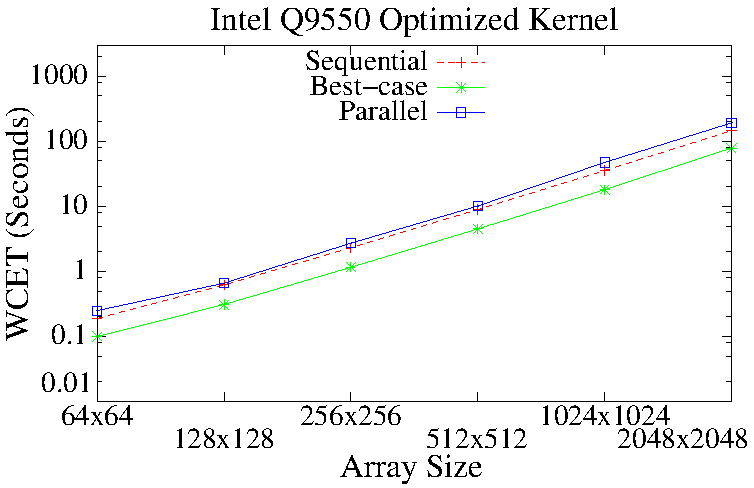
\includegraphics[scale=.4]{fig/q9550_optimized}
\label{fig:q9550_opt}
}
\caption{Benchmark evaluation on Intel dual-core Q9550 processor: (a) Original Linux kernel (b) Optimized Linux kernel.}
\label{fig:q9550_eval}
\end{figure}

We also ran the three applications in other two SMP processor, Intel Xeon 5030 and a PowerPC-based dual-core on the Cell architecture. Both use MESI as cache-coherence protocol and are UMA architectures. Figure~\ref{fig:xeon_ppc_eval} shows the benchmark performance on the two processors. We obtained even worse execution times, for the PowerPC processor the parallel version was up to 2.62 times slower than the sequential one, while for the Intel Xeon 5030 the parallel was up to 3.87 times slower. We also assigned threads to different cores in relation with their physical location (threads in the same physical die and threads in different physical dies\footnote{By using the \emph{proc filesystem} (/proc/cpuinfo) is possible to gather this information.}) and observed that there is almost no variation in the WCET for these SMP/UMA processors.

\begin{figure}[htb]
\centering
\subfigure[] {
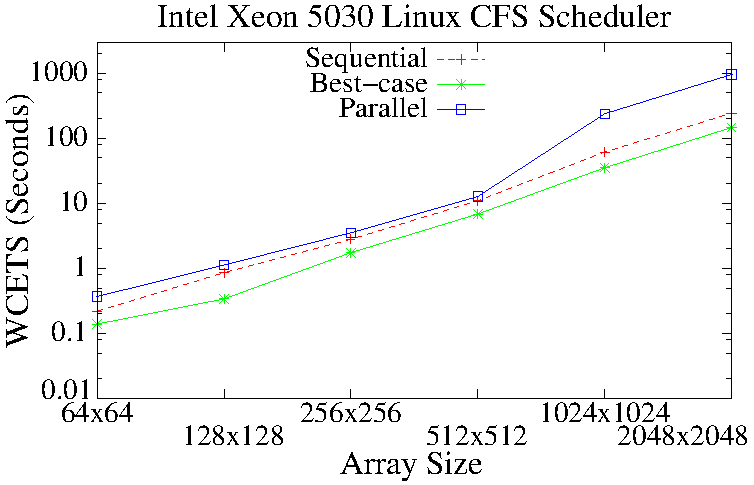
\includegraphics[scale=.4]{fig/xeon_5030}
\label{fig:xeon_5030}
}
\subfigure[] {
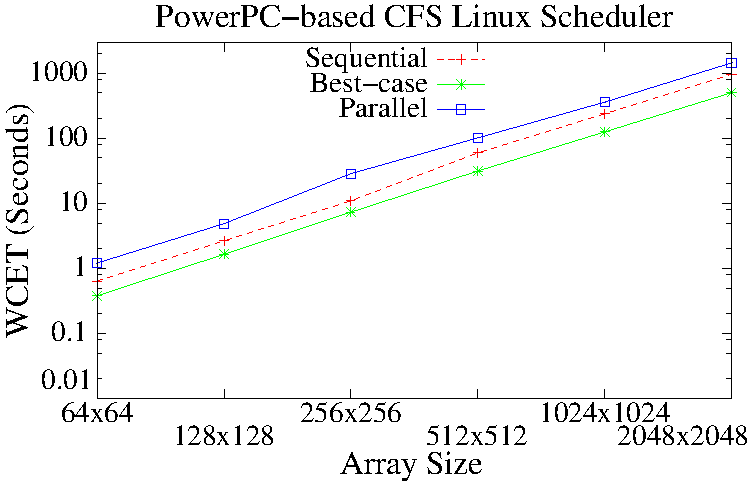
\includegraphics[scale=.4]{fig/powerpc_cpus_0_and_1}
\label{fig:ppc_0_and_1}
}
\caption{Benchmark evaluation on (a) Intel Xeon 5030 and (b) PowerPC-based processors.}
\label{fig:xeon_ppc_eval}
\end{figure}

Our next evaluation was carried out in the AMD Opteron 280 processor (see Table~\ref{tab:processors}). This processor implements MOESI as cache-coherence protocol and differ from the previous processors because it is a ccNUMA architecture. We evaluated three execution scenarios:

\begin{itemize}
	\item \textbf{Scenario 1}: threads running in cores in different dies (CPUS 0 and 1).
	\item \textbf{Scenario 2}: threads running in cores in the same die (CPUS 0 and 2).
	\item \textbf{Scenario 3}: Linux Completely Fair Scheduler (CFS) responsible for allocating a thread to a core. CFS uses a time-ordered rbtree to build a ``timeline" of future task execution. All runnable tasks are sorted by the a run-time key, which represents the expected CPU time a task should have. The scheduler gives the CPU to the leftmost task in the rbtree. The executed tasks are put into the tree more to the right, and thus giving the chance for every task to become the leftmost task within a deterministic amount of time. CFS supports the creation of groups of tasks, round-robin, FIFO, and real-time scheduling policies.
\end{itemize}

The objective of this test was to analyze the relation between the physical core location and the shared memory coherence by measuring the applications WCET. We assigned each thread in a specific core by using the \emph{pthread\_setaffinity\_np} function. Figure~\ref{fig:opt_0_and_1} shows the WCET for scenario 1. For arrays' size of 1024x1024 and 2048x2048 the sequential application was slightly faster than the parallel one. For all other sizes, the parallel one was slower than the sequential. In Figure~\ref{fig:opt_0_and_2} we present the measured WCET for scenario 2. In this scenario, the parallel version was always slower than the sequential one (up to 2.82 times using arrays' size of 64x64). We can also note a decreasing in the WCET as the arrays' size increase. Finally, Figure~\ref{fig:opt_cfs_linux} represents the measured WCET without assigning threads to any specific core, the CFS is responsible for assigning threads to cores. In this scenario, the applications performance was similar to the previous one. We can conclude that the WCET is related to the arrays' size, the bigger arrays' size the faster the execution time. Additionally, as expected from a ccNUMA architecture, there is a variation in the WCET when executing applications in cores physically located in different dies.

\begin{figure}[htb]
\centering
\subfigure[] {
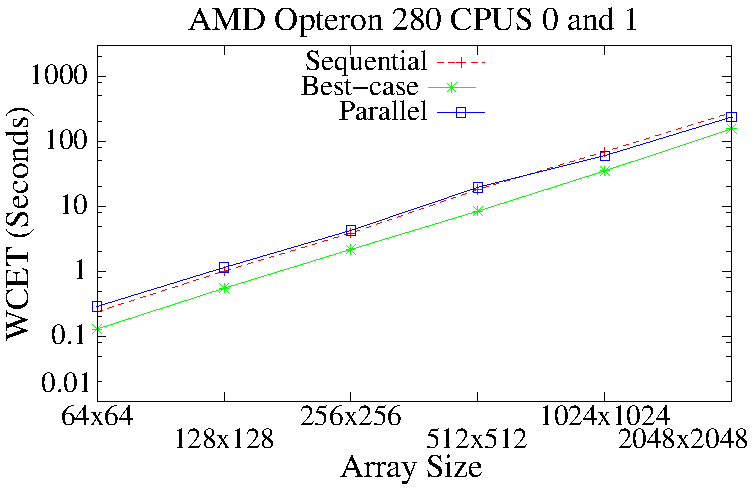
\includegraphics[scale=.4]{fig/opteron_cpus_0_and_1}
\label{fig:opt_0_and_1}
}
\subfigure[] {
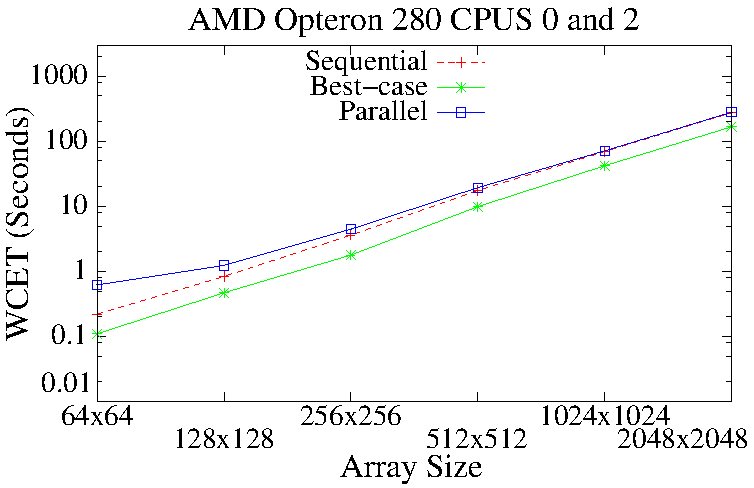
\includegraphics[scale=.4]{fig/opteron_cpus_0_and_2}
\label{fig:opt_0_and_2}
}
\subfigure[] {
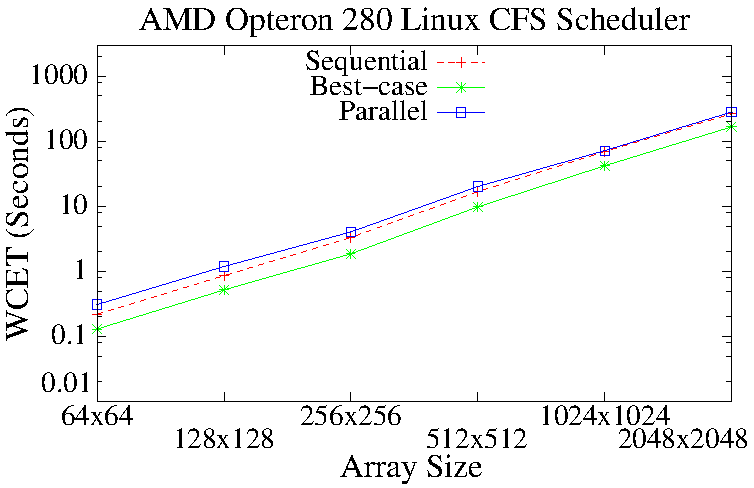
\includegraphics[scale=.4]{fig/opteron_cpus_random}
\label{fig:opt_cfs_linux}
}
\caption{Benchmark evaluation on AMD Opteron 280 processor assigning threads to specific cores: (a) CPUS 0 and 1 (b) CPUS 0 and 2 (c) Linux CFS scheduler.}
\label{fig:opteron_eval}
\end{figure}

Our next evaluation was carried out in the Intel i5-650 processor. This processor implements MESIF as cache-coherence protocol and it is also a ccNUMA architecture. We ran each application in three different scenarios:

\begin{itemize}
	\item \textbf{Scenario 1}: threads running in two different cores (CPUS 0 and 1).
	\item \textbf{Scenario 2}: threads running in the same core using \textit{Symmetric Multithreading} (SMT) technology (CPUS 0 and 2).
	\item \textbf{Scenario 3}: Linux CFS responsible for allocating a thread to a core.
\end{itemize}

Figure~\ref{fig:i5_eval} shows the WCET of each application in the three described scenarios. We can observe that the difference between the parallel and best-case WCET was basically the same in all scenarios. In scenario 2, the SMT obviously degrades performance of the parallel and best-case applications. In general, the parallel version was faster than the sequential one, only in scenario 1 with arrays' size of 2048x2048 it was slower than the sequential. This can be explained by the processor organization, composed by Intel's QuickPath Interconnect, and MESIF cache-coherence protocol.

\begin{figure}[htb]
\centering
\subfigure[] {
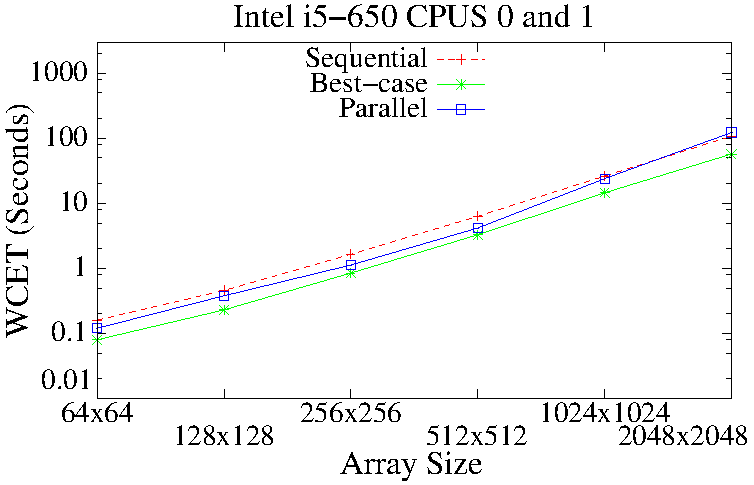
\includegraphics[scale=.4]{fig/intel-i5_cpus_0_and_1}
\label{fig:i5_0_and_1}
}
\subfigure[] {
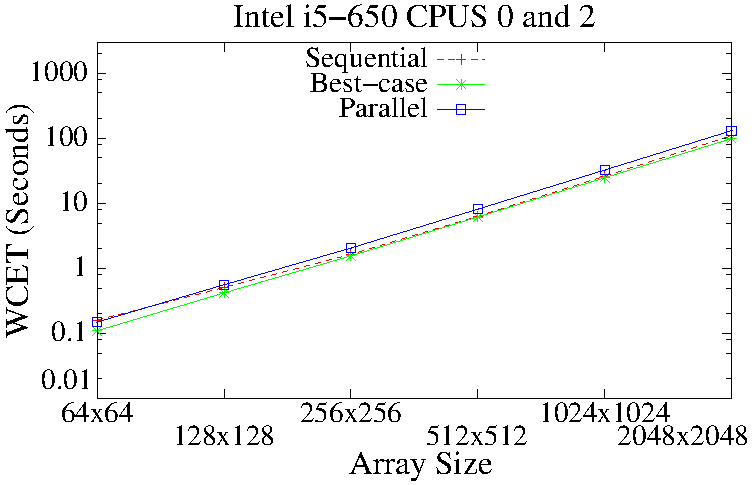
\includegraphics[scale=.4]{fig/intel-i5_cpus_0_and_2}
\label{fig:i5_0_and_2}
}
\subfigure[] {
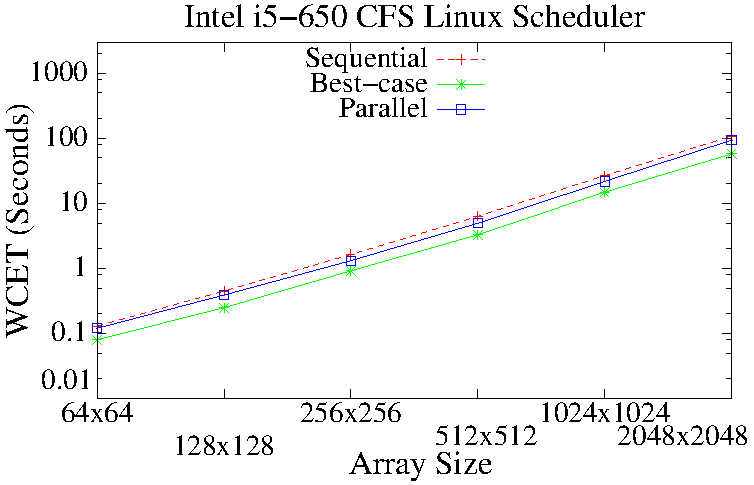
\includegraphics[scale=.4]{fig/intel-i5_cpus_random}
\label{fig:i5_cfs_linux}
}
\caption{Benchmark evaluation on Intel i5-650 processor assigning threads to specific cores: (a) CPUS 0 and 1 (b) CPUS 0 and 2 (c) Linux CFS scheduler.}
\label{fig:i5_eval}
\end{figure}

\section{Discussion and Future Work}
\label{sec:disc}
During our evaluations we observed a set of interesting facts regarding the described problem:

\textbf{SMP architectures.} We executed our benchmark on five different processors (Intel dual-core Q9550, PowerPC-based on Cell, Intel Xeon 5030, Intel i5-650, and AMD Opteron 280), that implement MESI, MESIF, and MOESI, as cache-coherence protocol, and have different memory organizations (ccNUMA and UMA). The five processors have proved that the impact of memory coherence is not negligible and should be mainly considered for real-time and processing intensive applications. The ccNUMA processors have suffered less impact considering the contention for shared data due to their bus, cache-coherence protocol, and memory organizations. We will concentrate our research in UMA systems that traditionally use MESI as memory coherency because they presented a worse degradation due to contention for shared memory. A execution time degradation up to 3.8 times for the parallel application was obtained using the Intel Xeon 5030 processor, which can certainly violate real-time guarantees if not correctly handled.

\textbf{Operating systems.} 
We used the Linux operating system. In general, OSes do not have any support for handling the contention for shared data. Moreover, the state-of-art real-time multicore scheduling algorithms do not consider the problem. Scheduling is a good alternative because is totally transparent to applications, there is no need to change APIs nor libraries, and can be easily integrated in RTOS.

\textbf{Memory partitioning/locking}. 
In order to reduce cache line invalidations and the interference among threads or other applications that do not share resources, methods such as memory partitioning and locking~\cite{Suhendra2008, Muralidhara:2010} could be used or easily solved by a special hardware support. However, in a cooperating real-time application, such as those found in digital signal processing area, where threads share data, a memory partitioning/locking do not solve the problem because threads will access the same data location on the memory hierarchy. Memory partitioning/locking can be used together with other techniques, such as scheduling, in order to decrease the contention for shared resources between several applications (inter-application contention) and application's threads (intra-application contention).

\textbf{Solution Statement}. Towards a solution for the problem, we envision a set of OS techniques designed together to provide predictability and real-time guarantees for embedded real-time applications. The proposed architecture is depicted in Figure~\ref{fig:proposed_solution} and it is a step forward to mitigate the effects of contention for shared memory. It is composed by a two-level OS cache partitioning to minimize the contention for cache space between different applications (inter-application partitioning) and between threads of the same application (intra-application partitioning)~\cite{Muralidhara:2010} and a shared memory-aware scheduler responsible for detecting and minimizing the influence of memory coherence from threads that share data (e.g. access serialization to the same cache line and saturation in the inter-core interconnection), while still compromising with real-time guarantees. Moreover, improved parallel programming techniques, such as \emph{sloppy counters}~\cite{BoydWickizer:10}, can also be incorporated into OS synchronization primitives.

\fig{proposed_solution}{Proposed solution architecture.}{scale=.6}

As embedded real-time systems usually have their requirements known at design time, it is possible to scan the source code and extract information about threads, including sharing data, with a specific tool~\cite{Cancian:07}, and use these information at run-time to help the scheduler decision. In addition, to monitor and detect patterns of threads memory accesses, and dynamically change the cache partitions size and decide when to take a scheduling decision related to threads that share data, the OS needs to gather information at run-time. HPCs are a good alternative for this purpose, since they are common in current multicore processors and the overhead for reading them is relatively low~\cite{Azimi:2009}. 

\begin{figure}[htb]
\centering
\begin{tabular}{cc}
	\subfigure[] {
	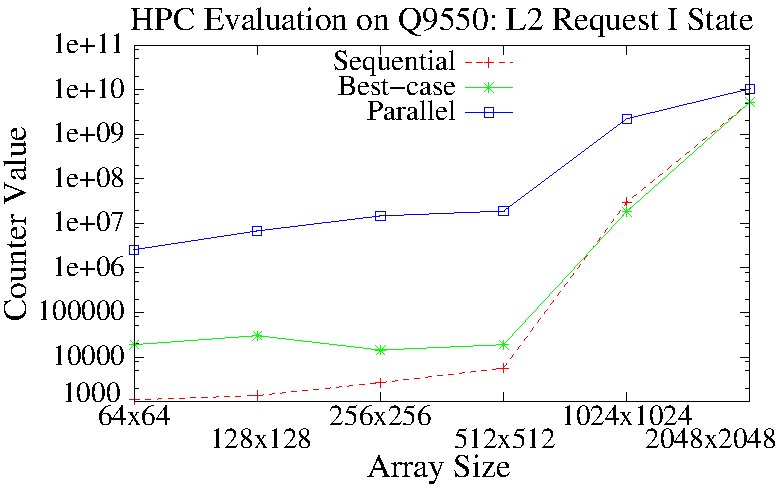
\includegraphics[scale=.3]{fig/HPC_l2_rqs_I_state}
	\label{fig:hpc_l2_i}} &
	\subfigure[] {
	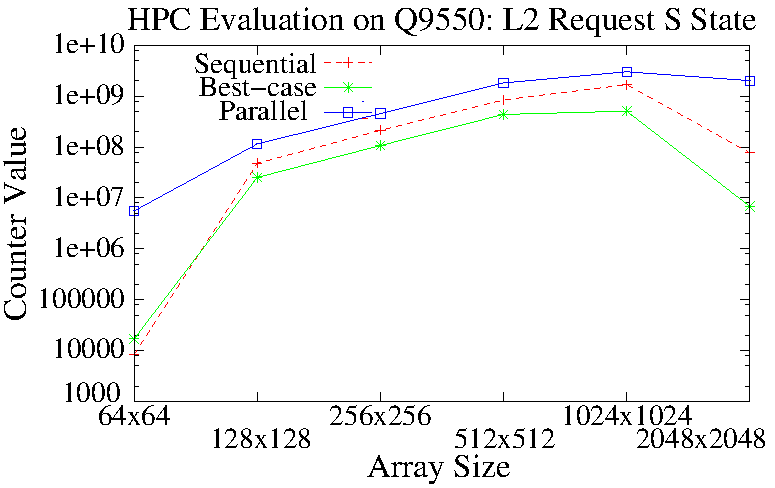
\includegraphics[scale=.3]{fig/HPC_l2_rqs_S_state}
	\label{fig:hpc_l2_s}
	}\\
	\subfigure[] {
	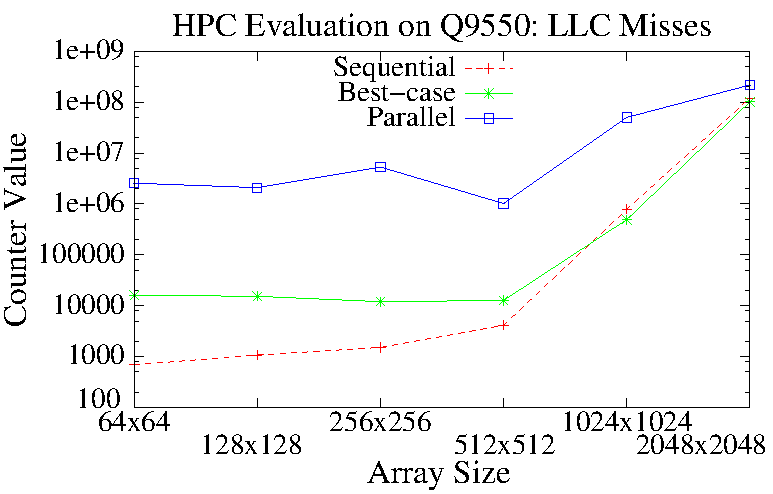
\includegraphics[scale=.3]{fig/HPC_llc_misses}
	\label{fig:hpc_misses}} &
	\subfigure[] {
	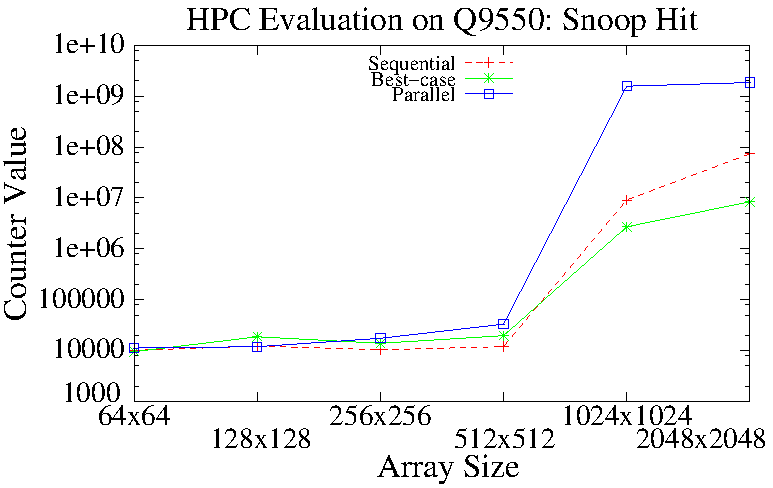
\includegraphics[scale=.3]{fig/HPC_snoop_hit}
	\label{fig:hpc_snoop_hit}
	}\\
	\subfigure[] {
	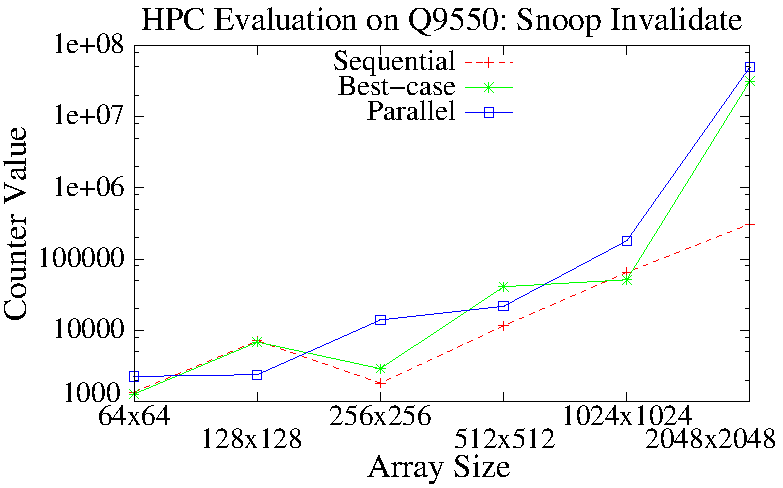
\includegraphics[scale=.3]{fig/HPC_snoop_invalidate}
	\label{fig:hpc_snoop_invalidate}} &
	\subfigure[] {
	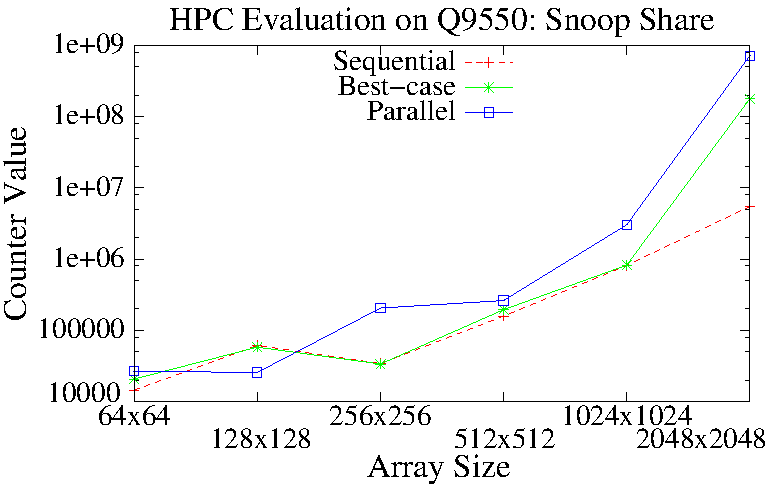
\includegraphics[scale=.3]{fig/HPC_snoop_share}
	\label{fig:hpc_snoop_share}
	}\\
	\multicolumn{2}{c}{
	\subfigure[] {
	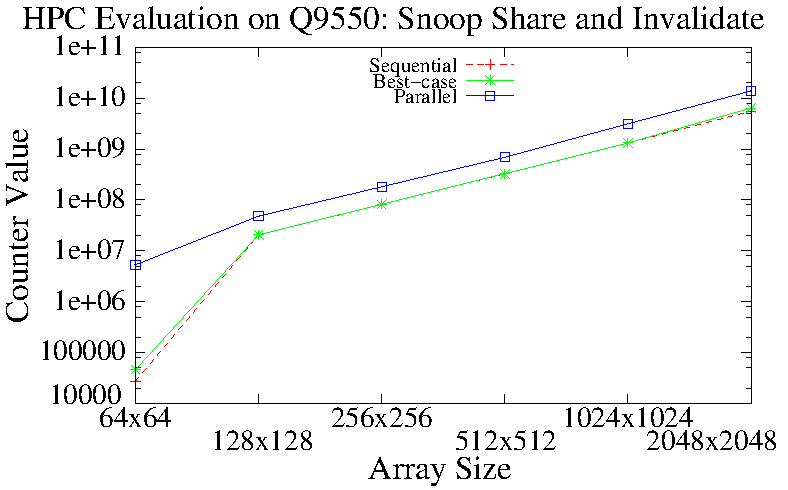
\includegraphics[scale=.3]{fig/HPC_snoop_share_invalidate}
	\label{fig:hpc_snoop_share_invalidate}
	}
	} \\
\end{tabular}
\caption{Benchmark HPCs evaluation on Intel Q9550 processor.}
\label{fig:HPC_eval}
\end{figure}

In this context, we present a preliminary analysis of HPCs running our benchmark in the Intel Q9550 processor. We use the \emph{perf} Linux tool to read the HPCs and the \emph{libpfm4} to list all available HPCs and use them as input to \emph{perf}. We ran each application for 10 times. Figure~\ref{fig:HPC_eval} shows the average value for each HPC: L2-cache request for I state, L2-cache request for S state, Last-Level Cache (LLC) misses, Snoop request hit, Snoop request Invalidate, Snoop request Share, and Snoop request Share and Invalidate. All HPCs are dependent of the application arrays' size. Snoop Hit, Snoop Invalidate, and Snoop Share have presented similar behavior for small arrays' size. As the arrays become bigger, the Snoop Hit has shown more variation between the parallel and the other two applications. Snoop Share and Invalidate has shown a constant behavior for the parallel version. L2-cache requests for I cache line state is a good alternative when the shared data is not too big. L2-cache requests for I and LLC misses had practically the same behavior. HPCs can be used to monitor the shared data addresses and mount a threads' sharing pattern with low overhead. An example is the \textit{shMap}, a vector of 8-bit saturating counters~\cite{Azimi:2009}. Each counter in the vector corresponds to a region in the virtual address space and its value is the representation of the sharing patterns detected inside that region. In summary, advanced HPCs capabilities allows the OS to have a precise view from applications' behavior and make smarter decisions at a fine granularity (e.g. cache line)~\cite{Azimi:2009}.

\section{Related Work}
\label{sec:related}

In the next subsections we summarize the main publications related to memory hierarchy in multicore systems and memory-aware and real-time multicore scheduling.

\subsection{Memory Hierarchy}

Shared cache partitioning is the most common method used to address contention and provide real-time guarantees to multicore applications. Partitioning is used to isolate applications workloads that interfere each other and thus increasing predictability. Several hardware-~\cite{Suhendra2008} and software-based~\cite{Cho:2006b, Zhang:2009, Muralidhara:2010} cache partitioning have been proposed in the last years. The software-based approach has the advantage to be completely transparent to applications and there is no need to special hardware support. The most common software-based technique is the \emph{page coloring}. This technique explores the translation from virtual to physical memory addresses presented in the virtual memory systems, in such a way that addresses from different applications are always mapped to pre-defined cache regions~\cite{Liedtke:1997, Cho:2006b}. Differently from the previous works, which focused on multi-application workloads, Chen analyzed different policies for managing shared caches for multi-threaded applications~\cite{YuChen:2009}. The work has shown that the shared-cache miss rate can be reduced by allocating a certain amount of space for shared data. A more sophisticated dynamic software-based partitioning technique that partitions the shared cache space between threads of a given application is proposed by Muralidhara~\cite{Muralidhara:2010}. At the end of each 15~ms interval, the dynamic cache partitioning scheme uses HPCs information, such as cache hit/misses, cycle and instruction counts for each thread, in order to allocate different cache space based on individual thread performance. The objective is to speed up the critical path, that is, the thread that has the slowest performance and, consequently, improve the overall performance for the application. The results have shown a performance gain of up to 23\% over a statically partitioned cache~\cite{Muralidhara:2010}. 

Cache partitioning can also be used together with some special hardware support, such as \textit{cache locking}~\cite{Suhendra2008}. Cache locking prevents data in the cache from being replaced at run-time, easing the schedulability analysis and obtaining predictability for real-time application~\cite{Suhendra2008}. However, in the most used current processors, there is no hardware support for cache locking. 

%Suhendra and Mitra propose the use of the shared cache in a restrictive manner in order to ease the schedulability analysis and obtain predictability for real-time application~\cite{Suhendra2008}. The proposal explores two mechanisms: \textit{cache locking} and \textit{cache partitioning}. The first one prevents data in the cache from being replaced at run-time. The second one assigns a partition of the cache to each task or processor and only allows cache replacement in the partitions. For both methods a special hardware support is needed, but in the most used current processors, there are no hardware support for cache partitioning/locking. The work suggests a set of guiding principles for designing a real-time system with respect of memory hierarchy.

%Considering the influence of memory hierarchy on predictability of real-time systems, Lars and Marwedel compare the effect of using cache or scratchpad memories on WCET analysis results~\cite{Marwedel2005}. They show that a scratchpad memory can obtain a more precise WCET. On the other hand, the difference between simulated average case execution time and WCET can grow larger for increasing cache sizes. As conclusion, they argue that scratchpad memories should be considered as feasible and worthwhile option during the design of time constrained systems, since they help to reduce the predicted WCET. However, several embedded systems do not feature a scratchpad memory.

Another important research topic related to memory hierarchy in multicore architectures is the timing and delay analyses. A framework for estimating the worst-case response time of tasks sharing an instruction cache was developed by Suhendra et al.~\cite{Li2009}. However, this work assumes that data memory references (i.e. data cache) do not interfere in the tasks' execution time. We have shown in this paper that the data memory hierarchy poses an important influence in the application's execution time. Moreover, the system model used by the authors is simple, it does not consider preemptions and data exchange among tasks are only done by message passing. \textit{Schedule-Sensitive} and \textit{Synthetic} are two methods to measure cache-related preemption and migration delays (CPMD)~\cite{Anderson2010a}. In the first method, delays are recorded online by executing tests and collecting the measured data. The drawback of this method is the impossibility of controlling when a preemption or migration happens, recovering many invalid data~\cite{Brandenburg2010a}. The second method tries to overcome this problem by explicitly controlling preemptions and migration of a task, and thus measuring the delays. The evaluation shows that the CPMD in a system under load is only predictable for working set sizes that do not trash the L2 cache~\cite{Anderson2010a}. Lars and Marwedel compare the effect of using cache or scratchpad memories on WCET analysis results~\cite{Marwedel2005}. They show that a scratchpad memory can obtain a more precise WCET. On the other hand, the difference between simulated average case execution time and WCET can grow larger for increasing cache sizes. As conclusion, they argue that scratchpad memories should be considered as feasible and worthwhile option during the design of time constrained systems, since they help to reduce the predicted WCET. However, several general-purpose and embedded systems do not feature a scratchpad memory.

\subsection{Memory-aware and Real-time Multicore Scheduling}

OS support for multicore applications, such as memory management, scheduling, and synchronization primitives, has received special attention in the last few years. For example, Corey~\cite{corey} and Barrelfish~\cite{Barrelfish} are two OS specifically designed to take full advantage of multicore processors. In addition, improvements on standard parallel programming techniques, such as proposed by \emph{sloppy counters}~\cite{BoydWickizer:10}, help on reducing the scalability problems found in the today's OS. Multicore scheduling algorithms focused on NUMA architectures are also an important research topic. Heterogeneity-Aware Signature-Supported (HASS) is a scheduling algorithm for Single-ISA heterogeneous multicore processors, which consist of cores with the same ISA, but different performance (e.g. clock frequency, power consumption, cache size)~\cite{Shelepov2009}. The algorithm is based on the idea of architectural signatures, a summary of architectural properties of an application. These information are used by the scheduler to match the application to a ``best" core. The architectural signatures are generated off-line and are embedded into the system's binary code. Initially, the algorithm does not support real-time applications. AMPS is another scheduler designed for NUMA architectures~\cite{Li2007}. The scheduler is composed by three components: (i) asymmetric-aware load balancing responsible for ensuring that each core has a proportional load depending on its computing power; (ii) faster-core scheduling ensures that threads will run on faster cores whenever they are under-utilized; and (iii) NUMA-aware migration that dynamically prevents thread migration in cores by using a thread resident set that contains the current pages in memory used by the thread. This resident set is used to estimate the migration overhead of a thread.

Several scheduling algorithms have been proposed in order to provide real-time guarantee for multicore applications. Brandenburg and Anderson discuss how the implementation of the ready queue, quantum-driven x event-driven scheduling, and interrupt handling strategies affect a global real-time scheduler~\cite{Anderson2009b}. The results indicate that implementation issues can impact schedulability as much as scheduling-theoretic tradeoffs. Moreover, in their case study, the best performance was achieved by using a fine-grained heap, event-driven scheduling, and dedicated interrupt handling. An empirical comparison of Global-EDF (G-EDF), Partitioned-EDF (P-EDF), and Clustered-EDF (C-EDF) on a 24-core Intel platform, assuming run-time overhead (e.g. release, context switch, and schedule times) and cache-related delay, has concluded that P-EDF outperforms the other evaluated algorithms in hard real-time scenarios~\cite{Brandenburg2010a}. Moreover, the same study suggests the use of ``less global" approaches (P-EDF and C-EDF-L2, which cluster at the cache level 2) in contrast of ``more global" approaches (G-EDF and C-EDF-L3) in hard real-time applications. A real-time scheduling for multiprocessors is proposed by Cho~\cite{Cho2006}. The authors proposed a new abstraction about task execution behavior on multiprocessors, named the time and local remaining execution-time plane (T-L plane). The entire scheduling over time is the repetition of T-L planes in various sizes. Consequently, a single T-L plane scheduling implies on feasible scheduling over all times. Another scheduling algorithm is presented by Srinivasan and Anderson~\cite{Srinivasan2006}. They show that the PD2 Pfair Algorithm is an optimal rate-based scheduling algorithm, since it correctly schedules any feasible intra-sporadic task system on M processors.

In the context of memory-aware real-time multicore scheduling algorithms, Calandrino and Anderson have proposed a cache-aware scheduling algorithm~\cite{Anderson2006, Anderson2008}. In their approach, the scheduling process is divided in two phases: (i) all tasks that may induce significant memory-to-L2 traffic are combined into groups off-line; and (ii) at run-time, a scheduling policy that reduces concurrency within groups is used. The paper introduces the concept of \emph{megatask}, which represents a task group and is treated as a single schedulable entity. All cores are symmetric, share a chip-wide L2 cache, and each core supports one hardware thread. Nevertheless, the algorithm fails in measuring the real influence of cache thrashing in an environment with threads sharing memory. $FP_{CA}$ is a cache-aware scheduling algorithm that divides the shared cache space into partitions~\cite{Guan2009}. Tasks are scheduled in a way that at any time, any two running tasks' cache spaces (e.g. a set of partitions) are non-overlapped. A task can execute only if it gets an idle core and enough cache partitions. The authors proposed two schedulability tests, one based on a linear problem (LP) and another one as an over-approximation of the LP test. Tasks are not preemptive and the algorithm is blocking, i.e. it does not schedule lower priority ready jobs to execute in advance of higher priority even though there are enough available resources. $FP_{CA}$ is executed whenever a job finishes or a new job arrives. 

Considering HPCs as an alternative to easily detect sharing pattern among threads and help scheduling decisions, Bellosa and Steckermeier were the first to suggest using HPCs to dynamically co-locate threads onto the same processor~\cite{Bellosa:1996}. Tam, Azimi, and Stumm use HPCs to monitor the addresses of cache lines that are invalidated due to cache-coherence activities and to construct a summary data structure for each thread, which contains the addresses of each thread that are fetching from the cache~\cite{Tam:2007}. Based on the information from this data structure, the scheduler mounts a cluster composed by a set of threads, and allocates a cluster to a specific core. However, this approach is not feasible for UMA processors, since there is no performance gains in allocating a thread to a specific core.

Another work to address shared resource contention via scheduling was proposed by Zhuravlev~\cite{Zhuravlev:2010}. The paper identifies the main problems that can cause contention in shared multicore processors (e.g. memory controller contention, memory bus contention, prefetching hardware, and cache space contention). The authors propose two scheduling algorithms (\textit{Distributed Intensity} - DI, and \textit{Distributed Intensity Online} - DIO). DI uses a threads' memory pattern classification as input, and distributes threads across caches such that the miss rates are distributed as evenly as possible. DIO uses the same idea, but it reads the cache misses online, through HPCs. DIO performed better than the Linux CFS both in terms of average performance as well as execution time stability from different executions~\cite{Zhuravlev:2010}.

In general, all the above related work do not consider a multicore system where threads share data. We demonstrated through our benchmark evaluation that the contention for shared memory data can influence the application's execution time and lead to performance degradation and deadline losses. 

\section{Conclusion}
\label{sec:conc}

This paper evaluated the real influence of contention for shared data memory in the context of real-time multicore applications. We have designed a worst-case benchmark in order to measure how the application's execution time is affected by the memory coherency hardware mechanism (e.g. snooping). The benchmark, composed by two versions of an application (sequential and parallel), was evaluated in 5 different processors with 3 different cache-coherence protocols (MESI, MOESI, and MESIF) and two memory architectures (UMA and ccNUMA). The results have shown that real-time applications on top of UMA processors must consider the coherence between the memory hierarchy. A execution time degradation up to 3.87 times in the parallel version was obtained only because the contention for shared memory data.

Our proposal towards a solution is a combination of OS techniques (e.g. inter- and intra-application memory partitioning, well-designed synchronization primitives, and a shared-aware real-time scheduling mechanism) in order to alleviate the effects of shared memory coherency (i.e. access serialization to the same cache line done by the cache coherence protocol and saturation into the inter-core interconnection). As future work, we will investigate techniques to be incorporated into the OS real-time scheduling.

\section{Acknowledgments}
This work was partially supported by the Coordination for Improvement of Higher Level Personnel (CAPES) grant, projects RH-TVD 006/2008 and 240/2008, and by the German Research Council (DFG) under grant no. SCHR 603/7-1.

% references section
\bibliographystyle{abbrv}
\bibliography{references}

% that's all folks
\end{document}
